
\documentclass{beamer}
\usepackage[utf8]{inputenc}

\usetheme{Madrid}
\usecolortheme{default}
\usepackage{amsmath,amssymb,amsfonts,amsthm}
\usepackage{mathtools}
\usepackage{txfonts}
\usepackage{tkz-euclide}
\usepackage{listings}
\usepackage{adjustbox}
\usepackage{array}
\usepackage{subcaption}
\usepackage{tabularx}
\usepackage{gvv}
\usepackage{lmodern}
\usepackage{circuitikz}
\usepackage{tikz}
\usepackage{graphicx}
\setbeamertemplate{page number in head/foot}[totalframenumber]
\usepackage[T1]{fontenc}
\usepackage{tcolorbox}
\tcbuselibrary{minted,breakable,xparse,skins}

\definecolor{bg}{gray}{0.95}
\DeclareTCBListing{mintedbox}{O{}m!O{}}{%
  breakable=true,
  listing engine=minted,
  listing only,
  minted language=#2,
  minted style=default,
  minted options={%
    linenos,
    gobble=0,
    breaklines=true,
    breakafter=,,
    fontsize=\small,
    numbersep=8pt,
    #1},
  boxsep=0pt,
  left skip=0pt,
  right skip=0pt,
  left=25pt,
  right=0pt,
  top=3pt,
  bottom=3pt,
  arc=5pt,
  leftrule=0pt,
  rightrule=0pt,
  bottomrule=2pt,
  toprule=2pt,
  colback=bg,
  colframe=orange!70,
  enhanced,
  overlay={%
    \begin{tcbclipinterior}
    \fill[orange!20!white] (frame.south west) rectangle ([xshift=20pt]frame.north west);
    \end{tcbclipinterior}},
  #3,
}

% Code style
\lstset{
    language=C,
    basicstyle=\ttfamily\small,
    keywordstyle=\color{blue},
    stringstyle=\color{orange},
    commentstyle=\color{green!60!black},
    numbers=left,
    numberstyle=\tiny\color{gray},
    breaklines=true,
    showstringspaces=false,
}

% Title info
\title %optional
{Analog - 1.1.18}
\date{March 30, 2026}
\author % (optional)
{EE25BTECH11018 - Darisy Sreetej}

\begin{document}

\frame{\titlepage}

\begin{frame}{Question}
 A Hilbert transformer is a :
 \begin{enumerate}

\item  Non $-$ linear system
\item  Non$-$causal system
 \item Time$-$varying system
\item Low$-$pass system

 \end{enumerate}
 \hfill(EC 2007) 
\end{frame}
\begin{frame}{Solution}

\textbf{Hilbert Transform} is defined as:\\[6pt]

\textbf{Time Domain:}\\[4pt]
The output (Hilbert transform) of any input $x(t)$ is given by convolution:

\begin{align}
    y(t) = x(t) * h(t) = \frac{1}{\pi} \int_{-\infty}^{\infty} \frac{x(\tau)}{t - \tau} \, d\tau
\end{align}

where , impulse response $h(t) = \frac{1}{\pi t}$ , $-\infty < t < \infty$


\end{frame}
\begin{frame}{Solution}
\textbf{Frequency Domain:}\\[4pt]
\begin{align}
H(j\omega) =
\begin{cases}
-j = e^{-j\frac{\pi}{2}}, & \omega > 0 \\
0, & \omega = 0 \\
+j = e^{j\frac{\pi}{2}}, & \omega < 0
\end{cases}
\end{align}

here, 
Magnitude :
$
|H(j\omega)| = 1 
$
\quad
Phase :
$
\angle H(j\omega) =
\begin{cases}
-90^\circ, & \omega > 0 \\
+90^\circ, & \omega < 0
\end{cases}
$
\end{frame}
\begin{frame}{Solution}
Let $x_1(t)$ , $x_2(t)$ be any two signals and $a$, $b$ be any scalars, 
then $y_1(t)$, $y_2(t)$ are the Hilbert transform outputs for the signals 
$x_1(t)$, $x_2(t)$ respectively:

\begin{align}
    y_1(t) = x_1(t) * h(t) &= \frac{1}{\pi} \int_{-\infty}^{\infty} 
    \frac{x_1(\tau)}{t - \tau} \, d\tau \\[4pt]
    y_2(t) = x_2(t) * h(t) &= \frac{1}{\pi} \int_{-\infty}^{\infty} 
    \frac{x_2(\tau)}{t - \tau} \, d\tau
\end{align}

Now, apply the Hilbert Transform to $ax_1(t) + bx_2(t)$ 
and let $z(t)$ be the output:

\begin{align}
    z(t) = \frac{1}{\pi} \int_{-\infty}^{\infty} 
    \frac{ax_1(\tau) + bx_2(\tau)}{t - \tau} \, d\tau
\end{align}

\end{frame}

\begin{frame}{Solution}

Using linearity of integration:

\begin{align}
z(t) &= \frac{1}{\pi} \int_{-\infty}^{\infty} \frac{ax_1(\tau)}{t - \tau} \, d\tau 
     + \frac{1}{\pi} \int_{-\infty}^{\infty} \frac{bx_2(\tau)}{t - \tau} \, d\tau \\[4pt]
     &= \frac{a}{\pi} \int_{-\infty}^{\infty} \frac{x_1(\tau)}{t - \tau} \, d\tau 
     + \frac{b}{\pi} \int_{-\infty}^{\infty} \frac{x_2(\tau)}{t - \tau} \, d\tau \\
     &= ay_1(t) + by_2(t)
\end{align}

Therefore, both additivity and homogeneity are satisfied by Hilbert Transform.
Thus, \textbf{Hilbert transform is linear}.

\end{frame}

\begin{frame}{Solution}

from (1) , for input $x(t)$
\begin{align}
y(t) = \frac{1}{\pi} \int_{-\infty}^{\infty} \frac{x(\tau)}{t - \tau}\, d\tau
\end{align}

on shifting the output :
\begin{align}
x_1(t) = x(t - t_0)
\end{align}

then , 
\begin{align}
y_1(t) = \frac{1}{\pi} \int_{-\infty}^{\infty} \frac{x(\tau - t_0)}{t - \tau}\, d\tau
\end{align}


Let:
\begin{align*}
\lambda = \tau - t_0 \\
\Rightarrow \quad \tau = \lambda + t_0 , \quad d\tau = d\lambda
\end{align*}




\end{frame}

\begin{frame}{Solution}


Substituting:
\begin{align}
y_1(t) = \frac{1}{\pi} \int_{-\infty}^{\infty} \frac{x(\lambda)}{t - (\lambda + t_0)}\, d\lambda \\
y_1(t) = \frac{1}{\pi} \int_{-\infty}^{\infty} \frac{x(\lambda)}{(t - t_0) - \lambda}\, d\lambda
\end{align}

On comparing with original output :

\begin{align}
y(t) = \frac{1}{\pi} \int_{-\infty}^{\infty} \frac{x(\lambda)}{t - \lambda}\, d\lambda
\end{align}

Thus,
\begin{align}
y_1(t) = y(t - t_0)
\end{align}

Hence, the Hilbert Transform is Time-Invariant
\end{frame}

\begin{frame}{Solution}
The impulse response of the Hilbert transformer is:
\begin{align}
h(t) = \frac{1}{\pi t}
\end{align}

For any $t < 0$, substitute a specific value, say $t = -1$:
\begin{align}
h(-1) = \frac{1}{\pi \cdot (-1)} = -\frac{1}{\pi} \neq 0
\end{align}

More generally, for \textit{any} $t < 0$:
\begin{align}
h(t) = \frac{1}{\pi t} \neq 0 \qquad \forall\; t < 0
\end{align}

since $\frac{1}{\pi t}$ is nonzero for all $t \neq 0$.

\begin{align}
\textbf{Required for causality:} & h(t) = 0 \quad \forall\; t < 0 \\[6pt]
\textbf{Actual impulse response:} & h(t) = \dfrac{1}{\pi t} \neq 0
\quad \forall\; t < 0
\end{align}

The condition is \textbf{not satisfied}.
\end{frame}

\begin{frame}{Solution}
  The output of the Hilbert transformer at time $t$ is:
\[
y(t) = \frac{1}{\pi} \int_{-\infty}^{\infty}
\frac{x(\tau)}{t - \tau}\, d\tau
= \frac{1}{\pi} \int_{-\infty}^{t} \frac{x(\tau)}{t-\tau}\,d\tau
\;+\;
\underbrace{\frac{1}{\pi} \int_{t}^{\infty}
\frac{x(\tau)}{t - \tau}\, d\tau}_{\text{depends on future input}}
\]

The second integral involves $x(\tau)$ for $\tau > t$, i.e., future
values of the input. This is a confirmation of non-causality.\\


Since $h(t) \neq 0$ for $t < 0$, the causality condition is violated: \\

The Hilbert transformer is a \textbf{Non-Causal} system.

\end{frame}

\begin{frame}{Solution}
    
For Low-pass system :
\begin{align}
|H(\omega)| = 1 \quad \text{for } |\omega| < \omega_c
\qquad \text{and} \qquad
|H(\omega)| = 0 \quad \text{for } |\omega| > \omega_c
\end{align}

For High-pass :
\begin{align}
|H(\omega)| = 0 \quad \text{for } |\omega| < \omega_c
\qquad \text{and} \qquad
|H(\omega)| = 1 \quad \text{for } |\omega| > \omega_c
\end{align}

For Band-pass :
\begin{align}
|H(\omega)| = 1 \quad \text{for } \omega_1 < |\omega| < \omega_2
\qquad \text{and} \qquad
|H(\omega)| = 0 \quad \text{elsewhere}
\end{align}

For All-pass :
\begin{align}
|H(\omega)| = 1 \quad \text{for all } \omega
\end{align}

The frequency response is:
\begin{align}
H(\omega) = -j \cdot \operatorname{sgn}(\omega)   \quad  \text{from (2)}
\end{align}



\end{frame}

\begin{frame}{Solution}
    Computing the magnitude response:
\begin{align}
|H(\omega)|
= \bigl|-j \cdot \operatorname{sgn}(\omega)\bigr|
= |-j| \cdot |\operatorname{sgn}(\omega)|
= 1 \cdot 1
= 1
\qquad \forall\; \omega \neq 0
\end{align}
\\
Since $|H(\omega)| = 1$ for all $\omega$, the all-pass condition is satisfied directly.

\quad

The Hilbert transformer is an \textbf{All-pass} system . \\

 \textbf{Conclusion :}

Thus , Hilbert transform is a linear time invariant , non-causal , all-pass system .

(option 2 is correct)

\end{frame}


\begin{frame}[fragile]
\frametitle{Python code}
    \begin{lstlisting}[language=Python]
import numpy as np
import matplotlib.pyplot as plt
from scipy.signal import hilbert

# example taken for time domain
fs       = 1000
T        = 1.0
t        = np.linspace(0, T, fs, endpoint=False)
x        = np.cos(2 * np.pi * 10 * t)
analytic = hilbert(x)
y        = np.imag(analytic)

# frequency domain
omega  = np.linspace(-10, 10, 10000)
H_real = np.zeros_like(omega)
H_imag = -np.sign(omega)
H_mag  = np.where(omega == 0, 0, 1)



\end{lstlisting}
\end{frame}
\begin{frame}[fragile]
    \frametitle{Python Code }
    \begin{lstlisting}[language=Python]
fig, axes = plt.subplots(2, 2, figsize=(14, 10))

# plot 1 
axes[0, 0].plot(t, x, color='royalblue', linewidth=2,label=r'$x(t) = \cos(2\pi \cdot 10t)$')
axes[0, 0].plot(t, y, color='crimson', linewidth=2, linestyle='--',label=r'$y(t) = \sin(2\pi \cdot 10t)$')
axes[0, 0].set_xlim(0, 0.2)
axes[0, 0].set_xlabel('$t$ (s)', fontsize=12)
axes[0, 0].set_ylabel('Amplitude', fontsize=12)
axes[0, 0].set_title(r'Time Domain — $x(t)$ and $y(t)$',fontsize=12)
axes[0, 0].legend(fontsize=9)
axes[0, 0].grid(True, alpha=0.3)

# plot 2
axes[0, 1].plot(omega, H_real, color='darkorange', linewidth=2,label=r'$\mathrm{Re}[H(\omega)] = 0$')

     \end{lstlisting}
\end{frame}
\begin{frame}[fragile]
    \frametitle{Python}
    \begin{lstlisting}[language=Python]
axes[0, 1].axhline(0, color='black', linewidth=0.6)
axes[0, 1].axvline(0, color='black', linewidth=0.5, linestyle='--', alpha=0.4)
axes[0, 1].set_xlim(-10, 10)
axes[0, 1].set_ylim(-1.8, 1.8)
axes[0, 1].set_yticks([-1, 0, 1])
axes[0, 1].set_xlabel(r'$\omega$', fontsize=12)
axes[0, 1].set_ylabel(r'$\mathrm{Re}[H(\omega)]$', fontsize=12)
axes[0, 1].set_title(r'Frequency Domain — $\mathrm{Re}[H(\omega)] = 0$',fontsize=12)
axes[0, 1].legend(fontsize=9)
axes[0, 1].grid(True, alpha=0.3)

# plot 3
axes[1, 0].plot(omega, H_imag, color='crimson', linewidth=2,
                label=r'$\mathrm{Im}[H(\omega)] = -\mathrm{sgn}(\omega)$')
axes[1, 0].plot(0, 0, 'ko', markersize=5)
axes[1, 0].axhline(0, color='black', linewidth=0.6)

    \end{lstlisting}
\end{frame}

\begin{frame}[fragile]
    \frametitle{Python code}

    \begin{lstlisting}[language=Python]
axes[1, 0].axvline(0, color='black', linewidth=0.5,linestyle='--', alpha=0.4)
axes[1, 0].set_xlim(-10, 10)
axes[1, 0].set_ylim(-1.8, 1.8)
axes[1, 0].set_yticks([-1, 0, 1])
axes[1, 0].set_xlabel(r'$\omega$', fontsize=12)
axes[1, 0].set_ylabel(r'$\mathrm{Im}[H(\omega)]$', fontsize=12)
axes[1, 0].set_title(r'Frequency Domain — $\mathrm{Im}[H(\omega)] = -\mathrm{sgn}(\omega)$',fontsize=12)
axes[1, 0].legend(fontsize=9)
axes[1, 0].grid(True, alpha=0.3)
axes[1, 0].annotate('+1', xy=(-9,  1.1), fontsize=10, color='crimson')
axes[1, 0].annotate('-1', xy=( 5, -1.2), fontsize=10, color='crimson')

# plot 4
axes[1, 1].plot(omega, H_mag, color='seagreen', linewidth=2.5,label=r'$|H(\omega)| = 1$')

    \end{lstlisting}
\end{frame}

\begin{frame}[fragile]
    \frametitle{Python code}

    \begin{lstlisting}[language=Python]
axes[1, 1].plot(0, 0, 'ko', markersize=5, label=r'$H(0) = 0$')
axes[1, 1].axvline(0, color='black', linewidth=0.5,
                   linestyle='--', alpha=0.4)
axes[1, 1].fill_between(omega, H_mag, alpha=0.12, color='green')
axes[1, 1].set_xlim(-10, 10)
axes[1, 1].set_ylim(-0.3, 1.8)
axes[1, 1].set_yticks([0, 0.5, 1.0])
axes[1, 1].set_xlabel(r'$\omega$', fontsize=12)
axes[1, 1].set_ylabel(r'$|H(\omega)|$', fontsize=12)
axes[1, 1].set_title(r'Magnitude — $|H(\omega)| = 1$ (All-pass)',
                     fontsize=12)
axes[1, 1].legend(fontsize=10)
axes[1, 1].grid(True, alpha=0.3)


plt.tight_layout()
plt.show()
\end{lstlisting}
\end{frame}
\begin{frame}{Plot}
    \begin{figure}
        \centering
        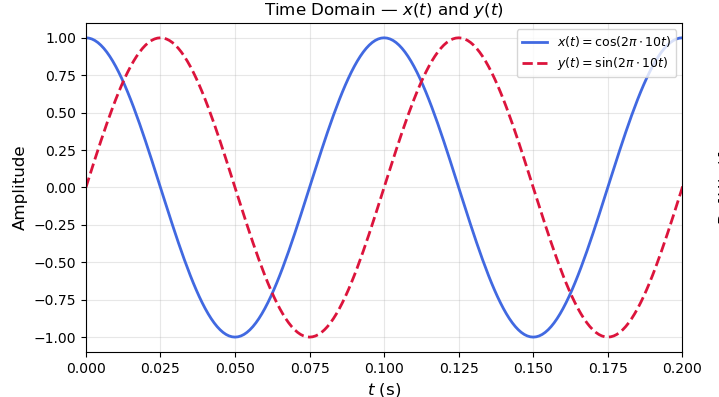
\includegraphics[width=0.89\linewidth]{1.png}
        \caption{Example taken $x(t) = \cos(2\pi \cdot 10t)$ }
        \label{fig:placeholder}
    \end{figure}
\end{frame}
\begin{frame}{Plot}
    \begin{figure}[htbp]
     \centering
     \begin{subfigure}[b]{0.55\textwidth}
         \centering
         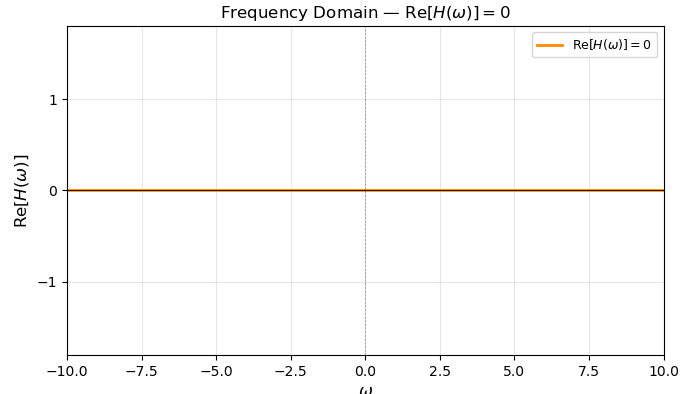
\includegraphics[width=\textwidth]{2.png}
     \end{subfigure}
     \hfill
     \begin{subfigure}[b]{0.55\textwidth}
         \centering
         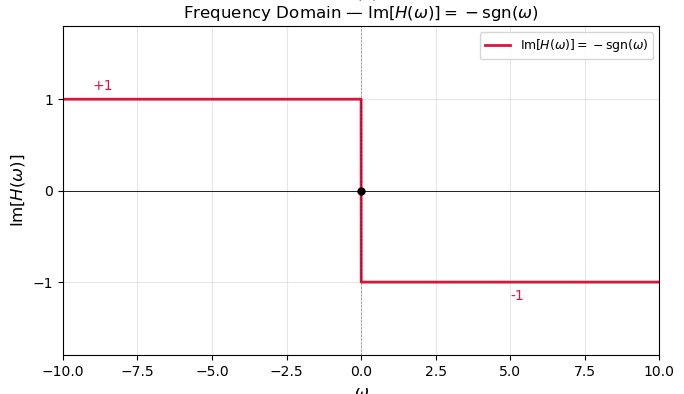
\includegraphics[width=\textwidth]{3.png}
     \end{subfigure}
\end{figure}
\end{frame}
\begin{frame}{Plot}
    \begin{figure}
        \centering
        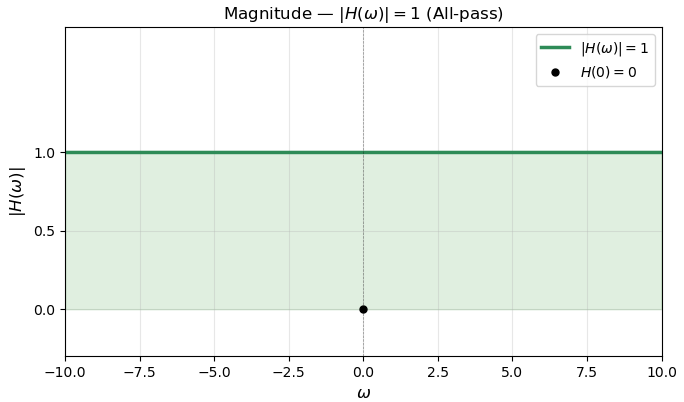
\includegraphics[width=1.02\linewidth]{4.png}
    \end{figure}
\end{frame}
\end{document}
\usepackage{subcaption}